\section{Definições}
\vspace{1cm}
A definição de $(\alpha,\lambda)$-limitada é inicialmente apresentada como uma propriedade pontual, assim como a definição de continuidade: \begin{definition} Sejam $\alpha, \lambda \ge 0$, $(X, d_X)$ e $(Y, d_Y)$ espaços métricos, $\mathcal{X} \subseteq X$. Uma função $f : \mathcal{X} \to Y$ é dita \textit{$(\alpha,\lambda)$-limitada no ponto $x \in \mathcal{X}$} quando, para todo $\tilde{x} \in \mathcal{X}$ tal que $d_X(x, \tilde{x}) \le \lambda$, temos $d_Y(f(x), f(\tilde{x})) \le \alpha$. \end{definition}

\begin{figure}[h!]
  \begin{center}
    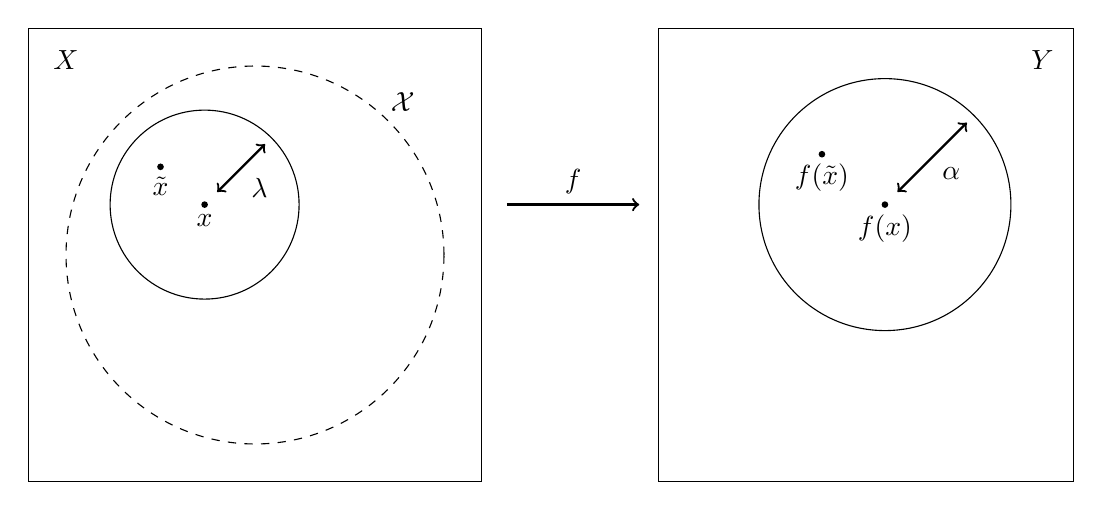
\begin{tikzpicture}[scale=.8]
      \node (X) at (-3, 3.1) {$X$};
      \node (Y) at (12.5, 3.1) {$Y$};

      \draw (-3.6, -3.6) rectangle (3.6, 3.6);
      \draw (6.4, -3.6) rectangle (13, 3.6);

      \fill (-0.8, 0.8) circle (1.5pt);
      \node[below] (x) at (-0.8, 0.8) {$x$};

      \fill (-1.5, 1.4) circle (1.5pt);
      \node[below] (xt) at (-1.5, 1.4) {$\tilde{x}$};

      \fill (10, 0.8) circle (1.5pt);
      \fill (9.0, 1.6) circle (1.5pt);
      \node[below] (y) at (10, 0.8) {$f(x)$};
      \node[below] (yt) at (9.0, 1.6) {$f(\tilde{x})$};

      \draw[dashed] (0, 0) ellipse (3cm and 3cm) node[above right, xshift=1.6cm, yshift=1.7cm] {$\mathcal{X}$};
      \draw[] (-0.8, 0.8) ellipse (1.5cm and 1.5cm);
      \draw[<->, thick] (-0.6, 1) -- ++(0.76, 0.76) node[midway, below right] {$\lambda$};
      \draw[] (10, 0.8) ellipse (2cm and 2cm);
      \draw[<->, thick] (10.2, 1) -- ++(1.1, 1.1) node[midway, below right] {$\alpha$};
      \draw[->, thick] (4, 0.8) -- (6.1, 0.8) node[midway, above] {$f$};
    \end{tikzpicture}
  \end{center}
  \captionsetup{justification=centering}
  \caption{
    \pt{Função $f : \mathcal{X} \to Y$ $(\alpha, \lambda)$-limitada em $x$.}
    \en{Function $f : \mathcal{X} \to Y$ which is $(\alpha, \lambda)$-bounded at $x$.}
  }
\end{figure}

\vspace{1cm}

\begin{definition} Sejam $\alpha, \lambda \ge 0$, $(X, d_X)$ e $(Y, d_Y)$ espaços métricos, $\mathcal{X} \subseteq X$. Uma função $f : \mathcal{X} \to Y$ é dita \textit{$(\alpha,\lambda)$-limitada} quando, para todo $x$ em $\mathcal{X}$, $f$ é $(\alpha,\lambda)$-limitada no ponto $x$. \end{definition}

Note que, para $\lambda = 1$, a definição acima estende naturalmente a condição de Hölder para a ordem $0$ e coeficiente $\alpha$ (veja \cite{holder}). Também é importante notar que muitos resultados de funções contínuas não se estendem para funções $(\alpha, \lambda)$-limitadas. Veja o exemplo \ref{vitali}.

Ao alterar a métrica, podemos considerar $\lambda = 1$ na definição acima sem perda de generalidade, porque $(X, d_X)$ é um espaço métrico se, e somente se, $(X, \lambda d_X)$ é um espaço métrico para todo $\lambda > 0$. Se desejarmos ter $d_X(x, \tilde{x}) \le \lambda$ para algum $\lambda > 0$, então podemos considerar o espaço métrico $(X, \frac{1}{\lambda} d_X)$ ao invés de $(X, d_X)$. Como nosso principal interesse neste trabalho são as funções $(k,1)$-limitadas, usaremos $\alpha$-limitada para denotar $(\alpha,1)$-limitada.

\begin{example} \label{vitali} Considere $V$ um conjunto de Vitali. A função $f : [0, 1] \to \mathbb{R}$, definida por $f(x) = 1_V$ se $x \in (0, 1)$ e $f(x) = 1 - x$ caso contrário, é $1$-limitada (considerando a métrica usual) mas não é contínua, não possui pontos fixos e não é Lebesgue integrável (veja \cite{vitali}). \end{example}

Toda função $f : X \to \mathbb{R}$ definida em um subconjunto discreto de $\mathbb{R}$ é contínua considerando a métrica induzida por $\mathbb{R}$, mas pode não ser $\alpha$-limitada para qualquer $\alpha > 0$. Veja a seguir.

\begin{example} \label{two_to_n} $f : \mathbb{Z} \to \mathbb{Z}$ dada por $n \mapsto 2^n$ não é $\alpha$-limitada (considerando a métrica usual) para nenhum $\alpha > 0$, pois $f(n + 1) - f(n) = 2^{n}$ é ilimitada. \end{example}

Abaixo estão alguns resultados imediatos da definição de $\alpha$-limitado.

\begin{theorem} Toda função $\alpha$-limitada é $(\alpha+\epsilon)$-limitada para todo $\epsilon > 0$. \end{theorem} \begin{proof} Evidente. \end{proof}

\begin{theorem} Sejam $(X, d_X)$ e $(Y, d_Y)$ espaços métricos, $\mathcal{X} \subseteq X$. Toda função Lipschitz contínua, com constante $K$, $f : \mathcal{X} \to Y$ é $K$-limitada. \end{theorem} \begin{proof} Para todo $x_1 \in \mathcal{X}$, $x_2 \in \mathcal{X}, d_X(x_1, x_2) \le 1$ e consequentemente $d_Y(f(x_1), f(x_2)) \le K d_X(x_1, x_2) \le K$. \end{proof}
Note que nem todas as funções $\alpha$-Hölder contínuas são $\beta$-limitadas para algum $\beta > 0$. A função $\sqrt{\cdot} : \mathbb{R}^+ \to \mathbb{R}$ constitui um contraexemplo (considerando a métrica usual) pelo mesmo motivo mencionado no exemplo \ref{two_to_n}.

\begin{theorem} Sejam $(X, d_X)$ e $(Y, d_Y)$ espaços métricos, $\mathcal{X} \subseteq X$, e $f : \mathcal{X} \to Y$ uma função. Se para todo $\epsilon > 0$ existe um $\alpha \in (0, \epsilon]$ tal que $f$ é $\alpha$-limitada, então $f$ é contínua. \end{theorem} \begin{proof} Com efeito, para cada $x \in \mathcal{X}, \epsilon > 0$, existe algum $\alpha \in (0, \epsilon]$ tal que $\tilde{x} \in \mathcal{X}, d_X(x, \tilde{x}) \le 1 \implies d_Y(f(x), f(\tilde{x})) \le \alpha \le \epsilon$. \end{proof}

\begin{theorem}
  Sejam $(X, d_X)$ e $(Y, d_Y)$ espaços métricos, $\mathcal{X} \subseteq X$. Se $(f_n) \to f$ ponto a ponto, $f_n : \mathcal{X} \to Y$ são $\alpha$-limitadas para todo $n \in \mathbb{Z}_{> 0}$, então $f$ é $\alpha$-limitada.
\end{theorem}
\begin{proof}
  Suponha, por contradição, que $f$ não seja $\alpha$-limitada. Então existem $x_1, x_2 \in \mathcal{X}$, $d_X(x_1, x_2) \le 1$, tal que $d_Y(f(x_1), f(x_2)) \coloneqq k > \alpha$. Como $(f_n) \to f$ ponto a ponto, existe algum $n \in \mathbb{Z}_{> 0}$ com $d_Y(f_n(x_1), f(x_1)) < \frac{k - \alpha}{2}$ e $d_Y(f_n(x_2), f(x_2)) < \frac{k - \alpha}{2}$. Consequentemente, $d_Y(f_n(x_1), f_n(x_2)) > k - \frac{k - \alpha}{2} - \frac{k - \alpha}{2} = \alpha$, uma contradição.
\end{proof}

As funções $\alpha$-limitadas podem não ser o limite pontual de qualquer sequência de funções contínuas.

\begin{example} A função de Dirichlet $1_\mathbb{Q} : [0, 1] \to \mathbb{R}$, também como função indicadora dos racionais, é $1$-limitada considerando a métrica usual de $\mathbb{R} \supset [0, 1]$, mas não é o limite pontual de nenhuma sequência de funções contínuas, pois é uma função da classe 2 de Baire (veja \cite{baire}). \end{example}

A aritmética com funções $\alpha$-limitadas não é a mesma que com funções contínuas definidas em $\mathbb{R}$.

\begin{theorem}
  Sejam $(X, d_X)$ e $(Y, d_Y)$ espaços métricos e $(Y, +Y, \cdot_Y)$ um espaço vetorial sobre $\mathbb{R}$. Se $f : X \to Y$ e $g : X \to Y$ são duas funções $\alpha$-limitadas, então $f + g$ é $(2\alpha)$-limitada e $\gamma f$ é $(\gamma \alpha)$-limitada para todo $\gamma > 0$.
\end{theorem}
\begin{proof}
  Se $x \in X$ e $\tilde{x} \in X$, $d_X(x, \tilde{x}) \le 1$, então $f(\tilde{x}) \in \overline{B}_{\alpha}(f(x))$ e $g(\tilde{x}) \in \overline{B}_{\alpha}(g(x))$, portanto $(f + g)(\tilde{x}) = f(\tilde{x}) + g(\tilde{x}) \in \overline{B}_{2\alpha}((f + g)(x))$, e consequentemente $f + g$ é $(2\alpha)$-limitada. Analogamente, $(\gamma f)(\tilde{x}) \in \overline{B}_{\gamma \alpha}(f(x))$ e $\gamma f$ é $(\gamma \alpha)$-limitada.
\end{proof}

O teorema acima permite considerar espaços vetoriais de mapas entre dois espaços métricos que são $\alpha$-limitados para algum $\alpha \ge 0$.

O produto de duas funções $\alpha$-limitadas (com o mesmo domínio e contradomínio) pode não ser $\beta$-limitado para nenhum $\beta > 0$, assim como o recíproco de uma função $\alpha$-limitada (quando definido).

\begin{example} $f : \mathbb{Z}_{> 0} \to \mathbb{Z}_{> 0}$ dada por $f(n) = n$ é $1$-limitada (considerando a métrica usual), mas $f^2$ coincide com $g : \mathbb{R} \to \mathbb{R}$, $g(x) = x^2$, portanto não é $\alpha$-limitada para nenhum $\alpha > 0$. \end{example}

\begin{example} $f : [1, +\infty) \to \mathbb{R}$ dada por $f(x) = \frac{1}{x^2}$ é $1$-limitada, mas $\frac{1}{f}$ coincide com $g : \mathbb{R} \to \mathbb{R}$, $g(x) = x^2$, portanto não é $\alpha$-limitada para nenhum $\alpha > 0$. \end{example}

O teorema de extensão para funções $\alpha$-limitadas não é muito forte.

Os exemplos abaixo ilustram por que as condições do teorema são necessárias.

\begin{example} Seja $X \coloneqq \{(x, \pm 1) \mid x \in \mathbb{Z}\} \subset \mathbb{Z}^2$. Considere $f : X \to \mathbb{Z}$ dada por $f(x, 1) = x$ e $f(x, -1) = 0$ para qualquer $x \in \mathbb{Z}$. Claramente, $f$ é $1$-limitada, considerando a métrica usual, mas $f$ não tem nenhuma extensão $\alpha$-limitada, para qualquer $\alpha > 0$, ao conjunto $\{(x, y) \mid x \in \mathbb{Z}, y \in \{-1,0,1\}\}$, pois $\overline{B}_1((x, 0)) \supset \{ (x, 1), (x, -1) \}$ e $f(x, 1) = x$, $f(x, -1) = 0$. \end{example}

\begin{figure}[H]
  \begin{center}
    \centering
    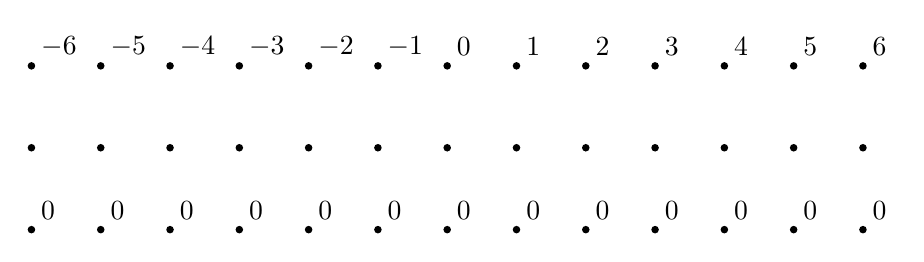
\begin{tikzpicture}[scale=0.8]
      \foreach \y in {1, 0, -1} {
          \foreach \x in {-6, ..., 6} {
              \fill[color=black] (\x*1.1+3,\y*1.3) circle (0.06);

              \ifnum\y=1
                \node[right] at (\x*1.1+3,\y*1.3+0.3) {$\x$};
              \fi
              \ifnum\y=-1
                \node[right] at (\x*1.1+3,\y*1.3+0.3) {$0$};
              \fi
            }
        }
    \end{tikzpicture}
    \captionsetup{justification=centering}
    \caption{
      \pt{Função $1$-limitada sem extensão $\alpha$-limitada, para qualquer $\alpha > 0$, para um conjunto com infinitos pontos adicionais.}
      \en{$1$-bounded function without an $\alpha$-bounded extension, for any $\alpha > 0$, for a set with infinitely many additional points.}
    }
  \end{center}
\end{figure}


\begin{example} Seja $s_n \in l^2(\mathbb{Z}_{> 0})$ a sequência com um $1$ na posição $n$-ésima e $0$'s nas outras posições, e $X = \{ s_n \mid n \in \mathbb{Z}_{> 0} \}$. $f : X \to \mathbb{Z}$ dada por $f(s_n) = n$ é $1$-limitada considerando a norma euclideana $l^2$, mas não tem nenhuma extensão $\alpha$-limitada ao conjunto $X \cup \{(0, 0, 0, \dots)\}$ para qualquer $\alpha \ge 0$. \end{example}

\begin{figure}[H]
  \begin{center}
    \begin{tikzpicture}
      \fill (0,0) circle (0.07);
      \node at ([shift={(1cm, -0.5cm)}] 0,0) {$(0, 0, \dots)$};

      % Constants
      \def\n{10} % Number of surrounding points
      \def\k{3.2}  % Constant k in the angle formula
      \def\startOffset{-77}

      % Loop to place points in a circular arrangement
      \foreach \i in {1,...,\n} {
          % Calculate angle for the point using (2 * pi / k) * log(N)
          \pgfmathsetmacro{\angle}{\startOffset + (360 / \k) * ln(\i + 1)}
          \pgfmathsetmacro{\angleout}{\startOffset + (360 / \k) * ln(\i)}


          % Coordinates of the surrounding point at radius 2
          \path (\angle:5) coordinate (P\i);
          \draw[dashed] (0, 0) -- (P\i);
          \ifnum\i>1
            \pgfmathtruncatemacro{\prev}{\i-1}
            % Calculate the start and end angles for each arc
            \pgfmathsetmacro{\startAngle}{\startOffset + (360 / \k) * ln(\prev + 1)}
            \pgfmathsetmacro{\endAngle}{\angle}
            \ifnum\i<4
              \draw[dashed]
              (P\prev) arc[start angle=\startAngle, end angle=\endAngle, radius=5]
              node[midway, above right] {\(\sqrt{2}\)}; % Label at midpoint of each edge
            \else
              \ifnum\i>4
                \draw[dashed]
                (P\prev) arc[start angle=\startAngle, end angle=\endAngle, radius=5];
              \else
                \draw[dashed]
                (P\prev) arc[start angle=\startAngle, end angle=\endAngle, radius=5]
                node[midway, above] {\(\sqrt{2}\)}; % Label at midpoint of each edge
              \fi
            \fi
          \fi


          % Draw the point and label it
          %\fill (P\i) circle (0.05) node[below left] {$s_{\i}$};

          \ifnum\i<5
            \fill[font=\bfseries] (P\i) circle (0.05) node[above left] {$s_{\i}$};
          \else
            \ifnum\i>9
              \fill (P\i) circle (0.05) node[below] {$s_{\i}$};
            \else
              \fill (P\i) circle (0.05) node[below left] {$s_{\i}$};
            \fi
          \fi
        }

      \node at ([shift={(0.5cm, -0.7cm)}] P10) {$\ddots$};

    \end{tikzpicture}
    \captionsetup{justification=centering}
    \caption{Sequência de pontos de $l^2(\mathbb{Z}_{> 0})$ na esfera unitária. A escala dos angulos que os pontos $s_n$ formam com o eixo $x$ é logarítimica em $n$.}
  \end{center}
\end{figure}


\begin{theorem} \label{tietze}
  Sejam $(X,d_X)$ e $(Y, d_Y)$ espaços métricos, $\mathcal{X}, \tilde{\mathcal{X}} \subset X$, onde $\tilde{\mathcal{X}}$ é finito, e seja $f : \mathcal{X} \to Y$ uma função $(\alpha,\lambda)$-limitada. Existe $\beta \ge 0$ tal que $f$ tem uma extensão $(\beta,\lambda)$-limitada para $\mathcal{X} \cup \tilde{\mathcal{X}}$ se e somente se $f$ é limitada em $\overline{B}_{\lambda}(\tilde{x}) \cap \mathcal{X}$ para cada $\tilde{x} \in \tilde{\mathcal{X}}$.
\end{theorem}

\begin{proof} A necessidade dessa condição é evidente. Vamos então provar que ela é suficiente.

  Podemos supor que $\tilde{\mathcal{X}} \cap \mathcal{X} = \varnothing$, já que obviamente $f$ é limitada em $\overline{B}_{\lambda}(x)$ para cada $x \in \mathcal{X}$.

  Procederemos por indução sobre o número $n$ de elementos em $\tilde{\mathcal{X}}$.

  Para $n = 0$, o resultado é óbvio. Suponha que o resultado seja verdade para $n$, e $\tilde{\mathcal{X}}$ tenha $n+1$ elementos.

  Fixe $\tilde{x} \in \tilde{\mathcal{X}}$ e $y \in Y$. Por hipótese, $f$ tem uma extensão $(\beta,\lambda)$-limitada para $\mathcal{X} \cup (\tilde{\mathcal{X}} \setminus {\tilde{x}})$. Defina $\tilde{f} : \mathcal{X} \cup \tilde{\mathcal{X}}$ por $\tilde{f}(\tilde{x}) = y$ e $\tilde{f}(x) = f(x)$ para cada $x \in \mathcal{X} \cup (\tilde{\mathcal{X}} \setminus {\tilde{x}})$. Claramente existe $\gamma \ge 0$ tal que $\tilde{f}$ é $(\gamma,\lambda)$-limitada em $x$ para cada $x$ diferente de $\tilde{x}$. Mas como $f$ é limitada em $\overline{B}_{\lambda}(\tilde{x}) \cap \mathcal{X}$, existe $M \ge 0$ tal que $\lvert f(x) \rvert \le M$ para cada $x \in \overline{B}_{\lambda}(\tilde{x}) \cap \mathcal{X}$. Portanto, $\lvert \tilde{f}(x)-\tilde{f}(\tilde{x})\rvert \le \lvert f(x)\rvert + \lvert -y\rvert \le M + \lvert-y\rvert$ para cada $x \in \overline{B}_{\lambda}(\tilde{x}) \cap \mathcal{X}$, e consequentemente, $\tilde{f}$ é $(\max\{M + \lvert-y\rvert, \gamma\},\lambda)$-limitada. Assim, o resultado também segue para $n+1$.
\end{proof}

Este corolário e os exemplos subsequentes ilustram algumas propriedades interessantes das funções $\alpha$-limitadas, especialmente como elas podem ser estendidas de um conjunto compacto para incluir finitos pontos adicionais.

\begin{corollary} Toda função $\alpha$-limitada definida em um conjunto compacto $\mathcal{X}$ possui uma extensão $\beta$-limitada para qualquer conjunto $\tilde{\mathcal{X}} \supseteq \mathcal{X}$ tal que $\tilde{\mathcal{X}} \setminus \mathcal{X}$ é finito. \end{corollary}

\begin{proof} Como $\mathcal{X}$ é compacto, o conjunto $\{ \overline{B}_1(x) \mid x \in \mathcal{X} \} \supseteq \mathcal{X}$ possui uma subcobertura finita, que naturalmente também cobre $\overline{B}_1(x) \cap \mathcal{X} \subset \mathcal{X}$ para todos os $x \in \tilde{\mathcal{X}} \setminus \mathcal{X}$. Assim pode-se tomar $\beta$ como o maior valor entre $\alpha$ e a variação máxima da extenção em cada um dos pontos adicionados. \end{proof}

Note que podemos ter $\beta < \alpha$ no teorema acima, já que $\alpha$ não precisa ser mínimo e $\tilde{\mathcal{X}} \setminus \mathcal{X}$ pode, por exemplo, ser vazio. Também não podemos assumir que $\beta = \alpha$ no teorema acima.

\begin{example} Seja $X \coloneqq \{-1, 1\} \subset \mathbb{Z}$. A função $f : X \to \mathbb{Z}$ dada por $f(x) = 2x$ é $1$-limitada (considerando a métrica usual), mas não existe uma extensão $1$-limitada de $f$ para o conjunto $\{-1, 0, 1\}$. \end{example}

O que foi apresentado neste capítulo mostra as propriedades básicas das funções $(\alpha,\lambda)$-limitadas e como elas se comportam em comparação com funções contínuas em espaços métricos. Os teoremas e exemplos ilustram as características fundamentais dessas funções, e fornecem uma base para o estudo aprofundado das funções $(\alpha,\lambda)$-limitadas em contextos mais específicos, como o explorado no terceiro capítulo.
